%
% File acl2021.tex
%
%% Based on the style files for EMNLP 2020, which were
%% Based on the style files for ACL 2020, which were
%% Based on the style files for ACL 2018, NAACL 2018/19, which were
%% Based on the style files for ACL-2015, with some improvements
%%  taken from the NAACL-2016 style
%% Based on the style files for ACL-2014, which were, in turn,
%% based on ACL-2013, ACL-2012, ACL-2011, ACL-2010, ACL-IJCNLP-2009,
%% EACL-2009, IJCNLP-2008...
%% Based on the style files for EACL 2006 by 
%%e.agirre@ehu.es or Sergi.Balari@uab.es
%% and that of ACL 08 by Joakim Nivre and Noah Smith

\documentclass[11pt,a4paper]{article}
\usepackage[hyperref]{acl2021}
\usepackage{times}
\usepackage{latexsym}
\renewcommand{\UrlFont}{\ttfamily\small}

% This is not strictly necessary, and may be commented out,
% but it will improve the layout of the manuscript,
% and will typically save some space.
\usepackage{microtype}
\usepackage{graphicx}

%\aclfinalcopy % Uncomment this line for the final submission
%\def\aclpaperid{***} %  Enter the acl Paper ID here

%\setlength\titlebox{5cm}
% You can expand the titlebox if you need extra space
% to show all the authors. Please do not make the titlebox
% smaller than 5cm (the original size); we will check this
% in the camera-ready version and ask you to change it back.

\newcommand\BibTeX{B\textsc{ib}\TeX}

% Standard package includes
\usepackage{times}
\usepackage{url}
\usepackage{latexsym}
\usepackage{graphicx}
\usepackage{xcolor}
\usepackage{longtable}
\usepackage{tikz}
\usetikzlibrary{calc}
\usepackage[draft]{todo}
\usepackage[normalem]{ulem}
\usepackage{xspace}
\usepackage{float}
\usepackage{amsmath,amsfonts,amssymb}
\usepackage{algorithm, algorithmic}
\newcommand{\fyTodo}[1]{\Todo[FY:]{\textcolor{orange}{#1}}}
\newcommand{\fyTodostar}[1]{\Todo*[FY:]{\textcolor{orange}{#1}}}
\newcommand{\fyDone}[1]{\done[FY]\Todo[FY:]{\textcolor{orange}{#1}}}
\newcommand{\fyFuture}[1]{\done[FY]\Todo[FY:]{\textcolor{red}{#1}}}
\newcommand{\fyDonestar}[1]{\done[FY]\Todo[FY:]{\textcolor{orange}{#1}}}
\newcommand{\revision}[1]{#1}
\newcommand{\revisiondel}[1]{}
\newcommand{\src}{\ensuremath{\mathbf{f}}} % source sentence
\newcommand{\trg}{\ensuremath{\mathbf{e}}} % target sentence
\newcommand{\domain}[1]{\texttt{\textsc{#1}}}
\newcommand{\system}[1]{\texttt{{#1}}}
\newcommand{\vlambda}{\ensuremath{\boldsymbol\lambda}\xspace} % parameters vector for a distribution
\newcommand{\indic}[1]{\ensuremath{\mathbb{I}(#1)}}
% \newcommand{\SB}[1]{\textcolor{green}{#1}}
% \newcommand{\SW}[1]{\textcolor{red}{#1}}
\newcommand{\SB}[1]{\textbf{#1}}
\newcommand{\SW}[1]{\underline{#1}}
% limits underneath
\DeclareMathOperator*{\argmin}{arg\,min}
\DeclareMathOperator*{\argmax}{arg\,max}
\renewcommand\textfraction{.1}
\renewcommand\floatpagefraction{.95}
\newcommand{\sbcl}[2]{{\scriptsize #1 \hfill $|$ \hfill  #2}}
\usepackage{multirow}
\usepackage{adjustbox}

\title{Improving Multi-Domain Neural Machine Translation with Differential Data Selection}

\author{First Author \\
  Affiliation / Address line 1 \\
  Affiliation / Address line 2 \\
  Affiliation / Address line 3 \\
  \texttt{email@domain} \\\And
  Second Author \\
  Affiliation / Address line 1 \\
  Affiliation / Address line 2 \\
  Affiliation / Address line 3 \\
  \texttt{email@domain} \\}

\date{}

\begin{document}
\maketitle
\begin{abstract}
  When building machine translation systems, one often needs to make the best out of heterogeneous sets of parallel data in training to achieve the best test performance in one or several domain(s) of interest. This multi-source (multi-domain) adaptation problem is often approached with instance selection or reweighting strategies, most of which pre-supposes an ad-hoc assessment of relevance for training sentences. In this contribution, we study the recently proposed Differential Data Selection (DDS) model  and explore its ability to serve an effective generic framework for these various situations. Our experiments for both domain adaptation and multi-domain learning show that DDS often enables to outperform heuristic training strategies; we also introduce a variant that boosts DDS performance of adapter-based multi-domain systems.
%   This is a well-known issue, which has given raise to a rich litterature in under the umbrellas of domain adaptation or multi-domain 

%   The priority of the in-domain performance in the overall evaluation affects the choice of choosing data. The problem falls in the data selection category in the domain adaptation topic. Several data selection methods pre-compute the domain-relatedness of training examples and use these scores to build mini-batches in the training while other works propose dynamic strategies to build training mini-batches based on reinforcement learning.
% In this study, we first formulate the most general algorithm for training the Neural Machine Translation (NMT) model given a predefined priority of the domains. Then, we apply a recently proposed method to solve the problem. We also report a disadvantage of DDS and fix it by proposing a minor development for DDS. Our experiments with a large sample of multi-domain systems show several important benefits of DDS in multi-domain NMT.
\end{abstract}

\section{Introduction}\label{sec:intro}
A typical setting in machine translation, is to collect the largest possible collection of parallel data for the chosen language pair, with the intent to achieve optimal performance for a task of interest. In such situations, the training data distribution is opportunistic, while the test data distribution is chosen; a key component in training is then to mitigate the detrimental effects of this mismatch between distributions. Single-source and multi-source domain adaptation is a well-studied instance of this setting (see \cite{Chu2017comparison} for a review) , and so is multi-domain learning \cite{Chu18multilingual,Zeng18multidomain,Jiang19multidomain}. A related situation is multi-lingual machine translation \cite{Firat16multiway,Ha16towards,Johnson17google,Arivazhagan19massively}\fyTodo{Add more recent work}, where the heterogeneity of training data not only corresponds to variation in topic or genre, but also in language.

\fyTodo{Label or covariate shift ?}
This problem is often approached with instance selection or reweighting strategies, where the available training data is used in proportion to its relevance for the chosen test conditions. Finding the optimal balance of training data is however a challenging task due for instance to similarity between domains / languages; it may also be suboptimal, as some domains or languages might be easier to train than others. Several recent proposals \cite{Wang17instance,Kumar19reinforcement, Wang20learning-multi} have explored ways to instead consider dynamic data selection strategy. We study in this contribution the proposal of \cite{Wang20balancing}, initially introduced for multilingual MT, with the goal to evaluate its potential in various single domain and multi-domain adaptation settings and assess DDS as an effective replacement to standard heuristics approaches.

Based on experimental results obtained on a diverse set of domains, our main conclusions are that (a) using DDS often yields overall performance that are as good as the standard fine-tuning strategy for domain adaptation; (b) DDS can effectively handle a variety of test target distributions without any meta-parameter search; (c) our extension of DDS is able to boost its performance when used in conjunction to the adapter model of \citet{Bapna19simple}.

% one often needs to make the best out of heterogeneous sets of parallel data in training to achieve the best test performance in one or several domain(s) of interest. This multi-source (multi-domain) adaptation problem is often approached with instance selection or reweighting strategies, most of which pre-supposes an ad-hoc assessment of relevance for training sentences. In this contribution, we study the recently proposed Differential Data Selection (DDS) model  and explore its ability to serve an effective generic framework for these various situations. Our experiments for both domain adaptation and multi-domain learning show that DDS often enables to outperform heuristic training strategies; we also introduce a variant that boosts DDS performance of adapter-based multi-domain systems.

\section{Learning with multiple data sources} \label{sec:mdmt}

We conventionally define a domain $d$ as a distribution $\mathcal{D}_d(x)$ over some feature space $\mathcal{X}$ that is shared across domains \cite{Pan10asurvey}: in machine translation, $\mathcal{X}$ is the representation space for input sentences; each domain corresponds to a specific source of data, and may differ from the other data sources in terms of textual genre, thematic content \cite{Chen16guided,Zhang16topicinformed}, register \cite{Sennrich16politeness}, style \cite{Niu18multitask}, etc. Translation in domain $d$ is formalized by a translation function $h_d(y|x)$ pairing sentences in a source language with sentences in a target language $y \in \mathcal{Y}$. $h_d$ is usually assumed to be deterministic (hence $y = h_d(x)$), but might differ from one domain to the other.

It is usual in MT to opportunistically collect training samples from multiple domains, which means that the training distribution $\mathcal{D}^s$ is a mixture $\mathcal{D}^s(x) = \sum_{d=1}^{n_d} \lambda^{s}_{d} \mathcal{D}_d(x)$\revision{, with $\{\lambda^{s}_d, d=1 \dots n_d\}$ the corresponding mixture weights such that $\sum_d \lambda^{s}_d=1$)}.

The main challenge is then to make the best of this heterogeneous data, with the aim to achieve the best possible system for the intended test conditions. These might correspond to data from just one of the training domains, as in standard supervised (multi-source) domain adaptation; a more difficult case is when the test data is from one domain unseen in training (unsupervised domain adaptation); in multi-domain adaptation the test distribution is itself a mixture of domains, some of which may also be observed in training.  Without loss of generality, one may then assume that the test distribution takes the form $\mathcal{D}^t(x) = \sum_d \lambda^{t}_{d} \mathcal{D}_d(x)$ - with only one non-null  $\lambda^{t}_{d}$ in the case of domain adaptation.
These situations are illustrated in Figure~\ref{fig:mdmt-lambdas}.
\begin{figure}[h]
  \centering
  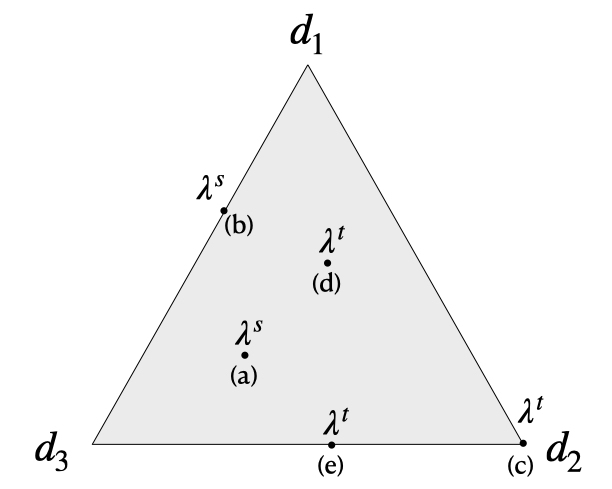
\includegraphics[width=0.48\textwidth]{mdmt-lambdas}
  \caption{Training and testing with distribution mismatch. We consider just three domains, and represent the mixture weights $\lambda^{s}$ and $\lambda^{t}$ in the 3-dimensional simplex. Training with weights in (a) and testing with weights in (c) is standard multi-source domain adaptation to $d_2$, while (b)-(c) is unsupervised adapation; training with weights in (a) and testing with weights in (d) is multi-domain learning, also illustrated with configurations (a)-(e) (training domain $d_1$ is not seen in test), and (b)-(d)  (test domain $d_2$ is unseen in training).}\label{fig:mdmt-lambdas}
\end{figure}

Theses situations have been amply documented from a theoretical perspective (eg.\ \cite{Mansour09multiple,Mansour09domainadaptation,Hoffman18algorithms}). A general recommandation in the DA setting  is to adjust the sampling distribution used to optimize the system so as to compensate for the mismatch between $\mathcal{D}^s(x)$ and $\mathcal{D}^t(x)$. This can be approximated by reweighting instances, or more conveniently domains, which are selected during training with a probability $Q^{trnn}(d)$, with $Q^{trn}(d) \neq \lambda^{s}(d)$.

Another practical standard approach to supervised DA is fine-tuning \cite{Luong15stanford,Freitag16fast}, where $q(x)$ is allowed to vary during the course of learning. With our notations, this approach amounts to first learning a initial parameter value with all data ($Q^{trn}(d) = \lambda^{s}(d)$), then to continue training with only batches from the test domain ($Q^{trn}(d) = \lambda^{s}(d) = \lambda^{t}(d)$). Note that this strategy may be suboptimal, since some out-of-domain samples may still be useful for the final performance due to eg.\ domain overlap. Optimizing the learning distribution in multi-domain learning is even more challenging, as the learner has to best take advantage of domain overlap, and also of the fact that some domains might be easier to learn than others.\fyTodo{How to measure this?} 

Differentiable data selection (DDS), introduced in \cite{Wang20optimizing} and later applied to multilingual machine translation in \cite{Wang20balancing}, introduces an additional degree of freedom and allows $Q^{trn}(d)$ to change more often in the course of training, as we now explain.

% === The part on multidomain training has been moved to the end.

\section{Differential Data Selection} \label{sec:dds}
We assume a training sample consisting of data from $n_d$ domains $d_1 \dots d_{n_d}$; we denote the size of the training subcorpus from domain $d$ as  $N^{trn}_d$, and $N^{trn} = \sum_d N^{trn}_d$ is the total number of training samples. We assume a fixed and pre-defined test distribution, approximated with an equivalent number of development corpora as $\widehat{\mathcal{D}^t}(x) = \sum_{d} Q^{dev}(d) \frac{[[x \in d]]}{N^{dev}_d}$, where $[[x \in d]]$ is the indicator function for domain $d$. Training is modeled as optimizing the parameters $\theta$ of a neural translation model.

Sampling training instances from a distribution $Q^{trn}(d)$ over domains results in a parameter estimate $\theta(Q^{trn})$, delivering performance that can be estimated using $Q^{dev}$. \cite{Wang20optimizing,Wang20balancing} then formulate the problem of finding an optimal sampling $Q^{trn}_{*}$ maximizing performance on the development data as the following bi-level optimization problem.
\begin{equation} \label{eq:bilevel}
\begin{split}
Q^{trn}_* &= \displaystyle{\mathop{\argmin}_{Q^{trn}} J(\theta^*(Q^{trn}), Q^{dev})} \\
					& \theta^*(Q^{trn}) = \displaystyle{\mathop{\argmin} J(\theta, Q^{trn})}, 
\end{split}
\end{equation}
where we use the following notations:\fyTodo{Overload Q, from domain to instances to pairs}
\begin{align*}
J(\theta, Q^{dev}) &= \displaystyle{\mathop{\sum}_{(x,y) \in Q^{dev}} l(\theta,x,y)} \\
J(\theta, Q^{trn}) &= \displaystyle{\mathop{E_{(x,y) \sim Q^{trn}}[l(\theta,x,y)]}} \\
l(\theta,x,y) &= - log P(\theta,x,y)
\end{align*}
Problem~\eqref{eq:bilevel} can be approached by coordinate gradient descent alternating between $Q^{trn}$ and $\theta$. \citet{Wang20balancing} limit the search space of $Q^{trn}$ to a parameterized differentiable function $Q^{trn}(\psi)$. Given $\psi_t$ at time step $s$, $\theta_t$ is updated via usual gradient descent as follows:
\begin{align*}
\theta_{t+1} &= \theta_t - \mathbf{lr}_{nmt} * \frac{\partial l(\theta_t, x,y)}{\partial \theta} \\
x,y &\sim Q^{trn}(\psi_t) \\
\end{align*}

Given $\theta_t$, $\psi_t$ is updated via the Reinforce algorithm:\fyTodo{Ref Reinforce}
\begin{align*}
  \psi_{t+1} &= \psi_t + \mathbf{lr}_{data} * R(x,y) * \\
  & \quad\quad \frac{\partial log(Q^{trn}(\psi_t)(x,y))}{\partial \psi} \\
x,y &\sim Q^{trn}(\psi_t) \\
R(x,y) &= \langle \frac{\partial l(\theta',x,y)}{\partial \theta}, \frac{\partial J(\theta_{t+1},Q^{dev})}{\partial \theta} \rangle \\
\theta' &= \theta_t - \mathbf{lr}_{nmt} * \frac{\partial l(\theta_t, x,y)}{\partial \theta} \\
\end{align*}

\fyTodo{Explain lr, may be more}
% To apply this method to multi-domain training (\system{Multi-DDS}), we limit the search family of training distribution $D_{trn}$ to the family of mixture of K in-domain training distribution such as $\sum_d \lambda^{s}_{d} \mathcal{D}_d(x,y)$. We also parameterize $\lambda^{s}_{d}$ using Softmax function so that $\lambda^{s}_{d} = \text{Softmax}(\psi)_d$ where $\psi \in \mathbb{R}^K$.

\section{Experimental settings} \label{sec:exp}
\subsection{Data and metrics \label{ssec:corpora}}
We experiment with translation from English into French and use texts initially originating from 6~domains, corresponding to the following data sources: the UFAL Medical corpus V1.0 (\domain{med})\footnote{\url{https://ufal.mff.cuni.cz/ufal_medical_corpus}. \revision{We only use the in-domain (medical) subcorpora: PATR, EMEA, CESTA, ECDC.}}, the European Central Bank corpus (\domain{bank}) \cite{Tiedemann12parallel}; The JRC-Acquis Communautaire corpus (\domain{law}) \cite{Steinberger06acquis}, documentations for KDE, Ubuntu, GNOME and PHP from Opus collection \cite{Tiedemann09news}, collectively merged in a \domain{it}-domain, Ted Talks (\domain{talk}) \cite{Cettolo12wit}, and the Koran (\domain{rel}). Complementary experiments also use v12 of the News Commentary corpus (\domain{news}). Most corpora are available from the Opus web site.\footnote{\url{http://opus.nlpl.eu}} These corpora were deduplicated and tokenized with in-house tools; statistics are in Table~\ref{tab:Corpora}. To reduce the number of types and build open-vocabulary systems, we use Byte-Pair Encoding \cite{Sennrich16BPE} with 30,000 merge operations on a corpus containing all sentences in both languages.\fyDone{Add \# number of tokens, also specificity ?}%

We randomly select in each corpus a development and a test set of 1,000 lines and keep the rest for training. Validation sets are used to chose the best model according to the average BLEU score \cite{Papineni02bleu}.\footnote{We use truecasing and the \texttt{multibleu} script.}\fyDone{A word about meta-parameter settings} Significance testing is performed using bootstrap resampling \cite{Koehn04statistical}, implemented in compare-mt\footnote{\url{https://github.com/neulab/compare-mt}} \cite{Neubig19compare-mt}. We report significant differences at the level of $p=0.05$.\fyDone{Fix correct p value}

%for contrast experiments, we also use supplementary test sets from three other domains: the official Khresmoi testset \cite{Khresmoi17test}, which is close to EMEA, News test 2014 \cite{Bojar14findings}, and IWSLT 2010 (Talk track) \cite{Paul10overview}. This enables us to evaluate the loss in performance when the test set is from a domain not seen in training.
% The model is also required to achieve comparable performance to generic model. To do so, we use newstest 2009 and IWSLT 2010 whose contain does not particularly belong to any domain.

\begin{table*}[htbp]
  \centering
  \begin{tabular}{|l|ccccccc|} %*{4}{|r|}}
    \cline{2-8} 
    %\multicolumn{4}{|l|}{Vocab size - En: 30,165, Fr: 30,398}\\
    \multicolumn{1}{c|}{} & \multicolumn{1}{c}{\domain{med}} & \multicolumn{1}{c}{\domain{law}} & \multicolumn{1}{c}{\domain{bank}} & \multicolumn{1}{c}{\domain{it}} & \multicolumn{1}{c}{\domain{talk}} & \multicolumn{1}{c}{\domain{rel}} & \multicolumn{1}{c|}{\domain{news}} \\
    \hline 
    \# lines & 2609 (0.68) & 501 (0.13) & 190 (0.05) & 270 (0.07) & 160 (0.04) & 130 (0.03) & 260 (0) \\
    \# \revision{tokens}  &  133 / 154  &  17.1 / 19.6 &  6.3 / 7.3 &  3.6 / 4.6 &  3.6 / 4.0 &  3.2 / 3.4 & 7.8 / 9.2   \\
    \# \revision{types}  & 771 / 720 & 52.7 / 63.1 & 92.3 / 94.7 & 75.8 / 91.4 & 61.5 / 73.3 & 22.4 / 10.5 & - \\
    \# \revision{uniq} & 700 / 640 & 20.2 / 23.7 & 42.9 / 40.1 & 44.7 / 55.7 & 20.7 / 25.6 & 7.1 / 2.1 & - \\
    \hline
  \end{tabular}
  \caption{Corpora statistics: number of parallel lines ($\times 10^3$) and proportion in the training domain mixture (which does not contain \domain{news}), number English and French tokens ($\times 10^6$), number English and French types ($\times 10^3$), number of types that only appear in a given domain ($\times 10^3$). \domain{med} is the largest domain, containing almost 70\% of the sentences, while \domain{rel} is the smallest, with only 3\% of the data.
  }
\label{tab:Corpora}
\end{table*}

\fyTodo{Keep this ?}
We measure the distance between domains using the $\mathcal{H}$-Divergence \cite{Ben-David09atheory}, which relates domain similarity to the test error of a domain discriminator: the larger the error, the closer the domains.
%Formally, given test sets of size $m$ for domains $A$ and $B$, and $h(x)$ a trained domain predictor, $\mathcal{H}(A,B)$ is computed %as:
%$$
%\mathcal{H}(A,B) = 2(1 - [\frac{1}{m} \sum_{x:h(x) = B} \mathbb{I}( x \in A) + \frac{1}{m} \sum_{x: h(x) = A} \mathbb{I}(x \in B)]),
% $$
% where $\mathbb{I}$ is the indicator function.
Our discriminator is a SVM independently trained for each pair of domains, with sentence representations derived via mean pooling from the source side representation of the generic Transformer model. We used the scikit-learn\footnote{\url{https://scikit-learn.org}} implementation with default values.\fyDone{Inform the classifier details}\fyDone{Insert tableau} Results in Table~\ref{tab:domaindist} show that all domains are well separated from all others, with \domain{rel} being the furthest apart, while \domain{talk} is slightly more central.

\begin{table}\centering
  \begin{tabular}{|l*{5}{|r}|} 
  \cline{2-6}
  \multicolumn{1}{c|}{} & \domain{law} & \domain{bank} & \domain{talk} & \domain{IT} & \domain{rel} \\ \hline
    \domain{med} &1.93 &1.97 &1.9 &1.93 &1.97 \\
    \domain{law}   && 1.94 & 1.97 &1.93 & 1.99 \\
    \domain{bank} &&&1.98 &1.94 &1.99 \\
    \domain{talk}   &&&&1.92 &1.93 \\
     \domain{IT}     &&&&& 1.99 \\ \hline
  \end{tabular}
  \caption{The $\mathcal{H}$-divergence between domains}
  \label{tab:domaindist}
\end{table}

\subsection{Baseline architectures \label{ssec:baseline}}
Our baselines are standard for multi-domain systems.\footnote{We however omit domain-specific systems trained only with the corresponding subset of the data, which are always inferior to the mix-domain strategy \cite{Britz17mixing}.} Using Transformers \cite{Vaswani17attention} implemented in OpenNMT-tf\footnote{\url{https://github.com/OpenNMT/OpenNMT-tf}} \cite{Klein17opennmt}, we build the following systems:

\begin{itemize}
\itemsep0em 
\item Generic models trained with various predefined mixtures of the training data taking the form:
\begin{align} \label{mixture:trn}
Q^{trn}(d) = \frac{q_d^{\alpha}}{\displaystyle{\mathop{\sum}_{d=1}^{n_d}q_d^{\alpha}}} &&
q_d = \frac{\mid N^{trn}_d \mid}{\displaystyle{N^{trn}}} % \mathop{\sum}_{i=1}^K\mid D_i \mid}}
\end{align} 
with $\alpha \in [0,0.25,0.5,0.75,1.0]$. We denote below these systems \system{Mixed-$\alpha$}
%on a concatenation of all corpora (\texttt{Mixed}). We develop two versions\footnote{In fact three: to enable a fair comparison with WDCMT, a RNN-based variant is also trained and evaluated. \revision{This system appears as \system{Mixed-Nat-RNN} in Table~\ref{tab:performance}}.} of this system, one where the domain unbalance reflects the distribution of our training data \revision{given in Table~\ref{tab:Corpora}} (\system{Mixed-Nat}) and one where all domains are equally represented in training (\system{Mixed-Bal}). The former is the best option when the train mixture $\mathcal{D}^s$ is also expected in testing; the latter should be used when the test distribution is uniform across domains. Accordingly, we report two aggregate scores: a weighted average reflecting the training distribution, and an unweighted average, meaning that test domains are equally important.
\item fine-tuned models \cite{Luong15stanford,Freitag16fast}, based on the \system{Mixed-$1.0$} system, further trained on each domain for at most 20~000 iterations, with early stopping when the dev BLEU stops increasing. The full fine-tuning (\system{FT-Full}) procedure may update all the parameters of the initial generic model, resulting in six systems adapted for one domain, with no parameter sharing across domains.

\item two multi-domain versions of the approach of \newcite{Bapna19simple}, denoted \system{FT-Res} and \system{MDL-Res}, where a domain-specific adaptation module is added to all the Transformer layers; within each layer, residual connections enable to short-cut this adapter. The former variant corresponds to the original proposal of \citet{Bapna19simple} (see also \cite{Sharaf20metalearning}). It fine-tunes the adapter modules of a \system{Mixed-$1.0$} system independently for each domain, keeping all the other parameters frozen. The latter uses the same architecture, but a different training procedure and learns all parameters jointly from scratch with the prefixed mixtures of training data \ref{mixture:trn}.
\end{itemize}

All models use embeddings and the hidden layers sizes of dimension~512. Transformers contain with 8 attention heads in each of the 6+6 layers; the inner feedforward layer contains 2048 cells. The adapter-based systems (see below) additionally use an adaptation block in each layer, composed of a 2-layer perceptron, with an inner $\operatorname{ReLU}$ activation function operating on normalized entries of dimension~1024. 
Training uses batches of~12,288 tokens, Adam with parameters $\beta_1=0.9$, $\beta_2= 0.98$, Noam decay ($warmup\_steps=4000$), and a dropout rate of $0.1$ in all layers.
\subsection{Multi-domain systems} \label{ssec:mdsys}
Our comparison of multi-domain systems includes our own reimplementations of recent proposals from the literature:\footnote{\revision{Further implementation details are in Appendix~A.}}
\begin{itemize}
\itemsep0em 
\item NMT models trained with Multi-DDS mixture given several objective testing distributions: uniform, uni-domain and natural.
\item \system{MDL-Res} trained from scratch with Multi-DDS mixture.
\end{itemize}

\section{Results and discussion \label{sec:results}}
\begin{table*}
  \centering% \small
  \begin{adjustbox}{width=2\columnwidth,center}
  \begin{tabular}{|p{3.0cm}|*{13}{r|}} \hline
    \multirow{2}{*}{Training} & \multicolumn{6}{|c}{$\lambda^t_d$} & \multicolumn{6}{|c|}{BLEU} & \multirow{2}{*}{BLEU} \\ \cline{2-13}	
  mixture & \multicolumn{1}{c|}{\domain{ med}} & \multicolumn{1}{c|}{\domain{ law}} & \multicolumn{1}{c|}{\domain{bank}} & \multicolumn{1}{c|}{\domain{talk}} & \multicolumn{1}{c|}{\domain{ it }} & \multicolumn{1}{c|}{\domain{ rel}} & \multicolumn{1}{c|}{\domain{ med}} & \multicolumn{1}{c|}{\domain{ law}} & \multicolumn{1}{c|}{\domain{bank}} & \multicolumn{1}{c|}{\domain{talk}} & \multicolumn{1}{c|}{\domain{ it }} & \multicolumn{1}{c|}{\domain{ rel}} & average \\
    \hline
  \system{Mixed-$0.0$} & 0.166&0.166 &0.166 &0.166 &0.166 & 0.166 & 35.26 &54.09 &52.49& 31.86& 44.94& 89.54& 51.36\\
  \system{Mixed-$0.25$} & 0.166&0.166 &0.166 &0.166 &0.166 & 0.166 &35.92& 54.87& 52.55& 32.55& 44.98& 90.28& 51.86\\
  \system{Mixed-$0.5$} & 0.166&0.166 &0.166 &0.166 &0.166 & 0.166 &36.11& 55.37& 51.76& 33.52& 46.23& 89.99& 52.16\\
  \system{Mixed-$0.75$} & 0.166&0.166 &0.166 &0.166 &0.166 & 0.166 &36.53&	55.03& 51.15& 33.98& 44.28& 87.22& 51.365\\
  \system{Mixed-$1.0$} & 0.166&0.166 &0.166 &0.166 &0.166 & 0.166 &37.33& 54.56& 50.05& 33.47& 43.23& 77.51& 49.36\\
  \system{Multi-DDS} & 0.166&0.166 &0.166 &0.166 &0.166 & 0.166 & & & & & & & \\
  \system{Multi-DDS-v1} & 0.166&0.166 &0.166 &0.166 &0.166 & 0.166 & & & & & & & \\
  \hline
  \end{tabular}
  \end{adjustbox}
\end{table*}
\begin{table*}
  \centering% \small
  \begin{adjustbox}{width=2\columnwidth,center}
  \begin{tabular}{|p{2cm}|*{13}{r|}} \hline
    \multirow{2}{*}{Training} & \multicolumn{6}{|c}{$\lambda^t_d$} & \multicolumn{6}{|c|}{BLEU} & \multirow{2}{*}{BLEU} \\ \cline{2-13}	
  mixture & \multicolumn{1}{c|}{\domain{ med}} & \multicolumn{1}{c|}{\domain{ law}} & \multicolumn{1}{c|}{\domain{bank}} & \multicolumn{1}{c|}{\domain{talk}} & \multicolumn{1}{c|}{\domain{ it }} & \multicolumn{1}{c|}{\domain{ rel}} & \multicolumn{1}{c|}{\domain{ med}} & \multicolumn{1}{c|}{\domain{ law}} & \multicolumn{1}{c|}{\domain{bank}} & \multicolumn{1}{c|}{\domain{talk}} & \multicolumn{1}{c|}{\domain{ it }} & \multicolumn{1}{c|}{\domain{ rel}} & average \\
    \hline
  \system{FT-Full} & 1.0 &0.0 & 0.0 &0.0 &0.0 & 0.0 &35.26 &54.09 &52.49& 31.86& 44.94& 89.54& 51.36\\
  \system{Multi-DDS} & 1.0 &0.0 & 0.0 &0.0 &0.0 & 0.0 &35.26 &54.09 &52.49& 31.86& 44.94& 89.54& 51.36\\
  \system{FT-Full} & 0.0 &1.0 & 0.0 &0.0 &0.0 & 0.0 &35.92& 54.87& 52.55& 32.55& 44.98& 90.28& 51.86\\
  \system{Multi-DDS} & 0.0 &1.0 & 0.0 &0.0 &0.0 & 0.0 &35.92& 54.87& 52.55& 32.55& 44.98& 90.28& 51.86\\
  \system{FT-Full} & 0.0 &0.0 & 1.0 &0.0 &0.0 & 0.0 &36.11& 55.37& 51.76& 33.52& 46.23& 89.99& 52.16\\
  \system{Multi-DDS} & 0.0 &0.0 & 1.0 &0.0 &0.0 & 0.0 &36.11& 55.37& 51.76& 33.52& 46.23& 89.99& 52.16\\
  \system{FT-Full} & 0.0 &0.0 & 0.0 &1.0 &0.0 & 0.0 &36.53&	55.03& 51.15& 33.98& 44.28& 87.22& 51.365\\
  \system{Multi-DDS} & 0.0 &0.0 & 0.0 &1.0 &0.0 & 0.0 &36.53&	55.03& 51.15& 33.98& 44.28& 87.22& 51.365\\
  \system{FT-Full} & 0.0 &0.0 & 0.0 &0.0 &1.0 & 0.0 &37.33& 54.56& 50.05& 33.47& 43.23& 77.51& 49.36\\
  \system{Multi-DDS} & 0.0 &0.0 & 0.0 &0.0 &1.0 & 0.0 &37.33& 54.56& 50.05& 33.47& 43.23& 77.51& 49.36\\
  \system{FT-Full} & 0.0 &0.0 & 0.0 &0.0 &0.0 & 1.0 &37.33& 54.56& 50.05& 33.47& 43.23& 77.51& 49.36\\
  \system{Multi-DDS} & 0.0 &0.0 & 0.0 &0.0 &0.0 & 1.0 &37.33& 54.56& 50.05& 33.47& 43.23& 77.51& 49.36\\
  \hline
  \end{tabular}
  \end{adjustbox}
  \label{tab:redomains}
\end{table*}
\section{Related Work \label{sec:related}}
\cite{Wang17instance} uses dynamic weighting (for sentences and domains) for DA.

\cite{Wang20multidomain} for multidomain DA.

\section{Conclusion and outlook \label{sec:discussion}}
\section*{Acknowledgments}
\bibliographystyle{acl_natbib}
\bibliography{multidomain}
%\appendix
\end{document}

Multi-domain learning, as defined in \citet{Dredze08online} further assumes that domain tags are also available in testing; the implication being that the test distribution is also as a mixture of several domains, making the problem distinct from mere domain adaption. A multi-domain learner is then expected to use these tags effectively \cite{Joshi12multidomain} when computing the combined translation function $h(x,d)$, and to perform well in all domains \cite{Finkel09hierarchical}. This setting is closely related to the multi-source adaptation problem formalized in \cite{Mansour09domainadaptation,Mansour09multiple,Hoffman18algorithms}.

This definition seems to be the most accepted view of a multi-domain MT\footnote{An exception is \citep{Farajian17multidomain}, where test translations rely on similarity scores between test and train sentences, rather than on domain labels.} and one that we also adopt here. In the absence of further specification, the naive answer to the MD setting should be to estimate one translation function $\hat{h}_d(x)$ separately for each domain, then to translate using $\hat{h}(x,d) = \sum_{d'} h_{d'}(x) \indic{d' = d}$, where $\indic{x}$ is the indicator function.

Given an objective mixture over test distribution $\lambda^{t}_{d}$,$d\in[1,\dots,K]$ and a mixture of training data $\lambda^{s}_{d}$, the Multi-domain training course is determined by the below algorithm \ref{alg:mdmt}. The training mixture can be constant or changing through time. Optimizing the training mixture is an interesting problem that we would like to address in the paper.

\begin{algorithm}[H]
\caption{Multi-domain Training} \label{alg:mdmt}
\label{alg:multidomain}
\begin{algorithmic}[1]
\REQUIRE {
\begin{itemize}
	\item Corpora $C^d, d\in [1,..,K]$ for $K$ domains equipped by an empirical distribution $D_d(x,y)$
	\item Dev sets $Dev^d, d\in [1,..,K]$ for $K$ domains.
	\item Testing mixture weights in the final evaluation $\lambda^t_d, d\in [1,..,K]$
	\item Batch size $B$.
	\item Temporal Data Selection Distribution(T-DSD)$$P_{\system{T-DSD}}(t)(x,y)=\sum_{d}\lambda^s_d(t)D_d(x,y)$$
	\item $Eval\_scores = []$
	\item $Early\_stopping$ criterion.
\end{itemize}}
\REPEAT 
\STATE{Iteration t.}
\STATE{Randomly pick $d \in [1,..,K]$ w.r.t  $[\lambda^s_1 \dots \lambda^s_K](t)$.}
\STATE{Sample $B$ sentences from $C^d$ with empirical distribution $D_d(x,y)$.}
\STATE{Update model by applying SGD computed from $B$ sampled sentences.}
\IF{$t \equiv 0 \mod{eval\_step}$}
	\STATE{Evaluate current model with $K$ dev sets. $S^t_d$ is the performance at iteration $t$ on domain $d$.}
	\STATE{Report weighted score using testing mixture weights $\lambda^t_d, d\in [1,..,K]$. $$eval(t) = \displaystyle{\mathop{\sum}_d \lambda^t_d S^t_d}$$}
	\STATE{$Eval\_scores.append(eval(t))$.}
\ENDIF
\IF{$Early\_stopping(Eval\_scores)$}
	\STATE{Stop training loop.}
\ENDIF
\UNTIL{convergence}
\end{algorithmic}
\end{algorithm}

